\section{Grundlagen}
\label{sec:grundlagen}

\subsection{Neuronale Netze}
\label{sec:neuronale-netze}

Neuronale Netze sind eine Modellklasse, welche zur L\"osung des
bereits ausf\"uhrlich
in~\cite{statistical_learning} beschriebenen Problems des statistischen
Lernens eingesetzt werden k\"onnen.
In dieser Problemsituation wird angenommen, dass sich der Zusammenhang zwischen
beobachtbaren Pr\"adiktorvariablen $X_1, ..., X_p$, welche sich durch
einen Vektor $X = (X_1, ..., X_p)$ zusammenfassen lassen, und einer
Zielvariable $Y$ durch eine Funktion $f^*$ mit $Y = f^*(X) + \epsilon$
modellieren l\"asst. Hierbei kann $\epsilon$ als eine zuf\"allige
St\"orgr\"o{\ss}e angesehen werden, die hier im weiteren Verlauf aber
keine wichtige Rolle spielt.
Das Ziel von Neuronalen Netzen ist es, die unbekannte Funktion $f^*$
zu approximieren.

Die folgenden Erkl\"arungen zum Aufbau und zum Training neuronaler Netze
st\"utzen sich wesentlich auf~\cite{Goodfellow-et-al-2016} und sind hier
auf das grundlegendste reduziert.

\subsubsection{Aufbau}

Wie in~\ref{sec:neuronale-netze} angedeutet, definiert ein neuronales Netz
also eine Abbildung $f$, welche den Zusammenhang zwischen einer Eingabe $X$
und einer Ausgabe $Y$ approximieren soll.
Eine Hauptcharakteristik von neuronalen Netzen ist es, dass die Funktion $f$
durch die Verkettung weiterer Funktionen gebildet wird.
Ist ein neuronales Netz beispielsweise durch
$f(x) = f^{(3)}(f^{(2)}(f^{(1)}(x)))$ gegeben, so setzt es sich aus der
Verkettung der einzelnen Funktionen $f^{(1)}$, $f^{(2)}$ und
$f^{(3)}$ zusammen. Wie genau diese Funktionen aussehen k\"onnen, soll an dieser
Stelle bewusst ersteinmal offen bleiben.

Solche Ketten von Funktionen k\"onnen gut durch
azyklische Graphen beschrieben werden. Hierbei wird jedes Zwischenergebnis
durch einen Knoten repr\"asentiert, jede Kante zwischen zwei Knoten beschreibt
die Operation, die vom einen Ergebnis zum n\"achsten gef\"uhrt hat.
Der Beispielgraph zu $f(x) = f^{(3)}(f^{(2)}(f^{(1)}(x)))$ ist in
Abbildung~\ref{fig:einfacher-graph} zu sehen.

\begin{figure}[h]
    \centering
    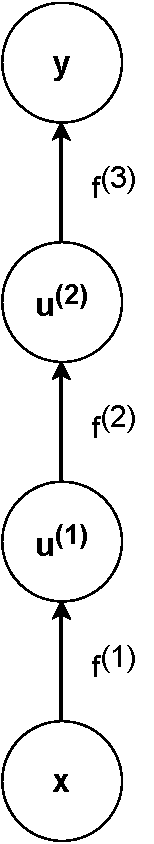
\includegraphics[height=0.25\textheight]{abbildungen/basic_network_graph}
    \caption{Verkettung dreier Funktionen dargestellt als azyklischer Graph.}
    \label{fig:einfacher-graph}
\end{figure}

Im Kontext von neuronalen Netzen wird jede der Funktionen
$f^{(1)}$, $f^{(2)}$ und $f^{(3)}$ auch als eine \textbf{Schicht} im
neuronalen Netz bezeichnet.
Da $f^{(1)}$ und $f^{(2)}$ im Inneren des Netzwerks liegen, bezeichnet man
diese Schichten auch als \textbf{versteckte Schichten}.

\subsubsection{Training}

\subsubsection{Convolutional Neural Networks}

\subsection{OpenCV}

\subsection{Tesseract}